\clearpage % clear the prior chapter's page

\chapter{\mytool: Usage, Architecture, Implementation Details, and Features}\label{CH4_ToolUsage}
%\vspace{-7mm}
%\bigskip


\section{Usage}
For ease of this experiment, we have created a tool, \mytool~\cite{weber_2022}, that will simplify the unit tests. To use this tool, the developer will only have to provide the following: test file with full path, name of the test (as a single file can have many tests and we may want to reduce only one failing test), and the path of the \texttt{.csproj} file associated with the code. All of this information is already available to the developers. Optionally, the developer can provide a particular folder path if they want to use it to store intermediate results and the final output in that folder. The architecture from a developer's perspective is described in figure~\ref{fig:tool_architecture}. If you compare the architecture figure with the \emph{Perses} workflow figure and the \emph{Picireny} architecture figure, the contrast is clear~\cite{hodovan2016modernizing, perses}. Both the \emph{Perses} and \emph{Picireny} approaches require significant preprocessing steps that require other libraries, toolsets, and components. Both of them require a test script to be available, normally a shell file or a batch file. \mytool does not require any of these as explained in the architecture section. 

\section{Architecture}
As \mytool is implemented for C\#, it takes into consideration how C\# programs are organized using \texttt{.sln} and \texttt{.csproj} files. In order to compile or run the test, \mytool uses the \texttt{.csproj} file, the test, and the built-in build+run utility available as part of the \texttt{.NET} framework and Roslyn compiler to generate the necessary build+run script. The process is described in the right side of figure~\ref{fig:internal}. On the left side, we describe how a test is processed first using the Roslyn compiler to generate the parse tree. The parse tree will go through a pruning and transformation process to produce a tree where \emph{Tree} statements will be processed as \emph{NonTree} statements. The test, the processing statement list, and the build+run script will then be passed to the DD algorithm to produce the minimized test. The \emph{Perses} and \emph{Picireny} approaches require the user of their tool to provide a test script which may increase in complexity over time as both approaches will require a new test script for each test minimization. 


\section{Implementation}
A great effort was made to not have any external dependencies, libraries, or tool sets and, as a result, \mytool only utilizes the \texttt{.NET} framework and Roslyn compiler API, which is available as part of the \texttt{Microsoft.CodeAnalysis} library. Therefore, a user can easily invoke \mytool as a command line utility without the needing to download or maintain any external components or libraries. Because \mytool is a C\# specific tool designed for C\# unit tests, the need for preprocessing steps is eliminated.


\begin{center}
\begin{figure}[!ht]
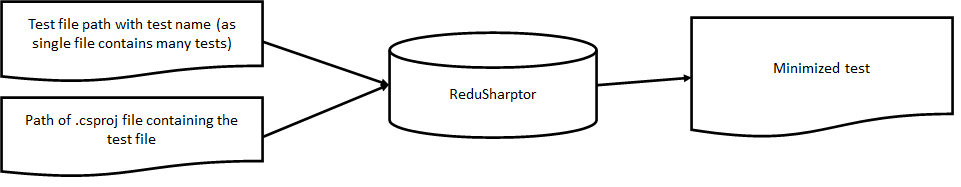
\includegraphics[width=\linewidth]{tool_archicture.png}
\caption{\mytool architecture from a user's perspective}
\label{fig:tool_architecture}
\end{figure}
\end{center}

\begin{center}
\begin{figure}[!ht]
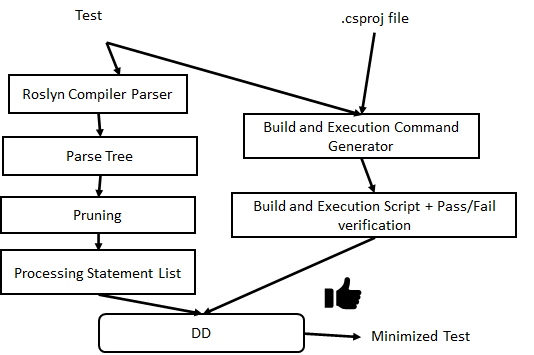
\includegraphics[width=\linewidth]{internal_architecture.png}
\caption{\mytool internal architecture with implementation details}
\label{fig:internal}
\end{figure}
\end{center}


\begin{figure}
\begin{lstlisting}[language=C, linewidth=0.6\linewidth]
[Fact]
public void Foo()
{
	Math m = new Math();  // 1
	Assert.Equal(m.Add(3,4),7);  // 2
	if(true){  // 3
		Assert.Equal(m.Add(4,5),9);  // 4
	}  // 5
}
\end{lstlisting}
\caption{\texttt{foo} test to demonstrate AST}
\label{fig:foo}
%\vspace{-0.5in}
\end{figure}


\begin{figure*}
\begin{lstlisting}
ReduSharptor.exe ".\language-ext\LanguageExt.Tests\ApplicativeTests.cs" "ListCombineTest" ".\language-ext\LanguageExt.Tests\LanguageExt.Tests.csproj" ".\Simplified Test Results"
\end{lstlisting}
\caption{\texttt command line execution of \mytool}
\label{fig:foo}
%\vspace{-0.5in}
\end{figure*}


\begin{figure*}
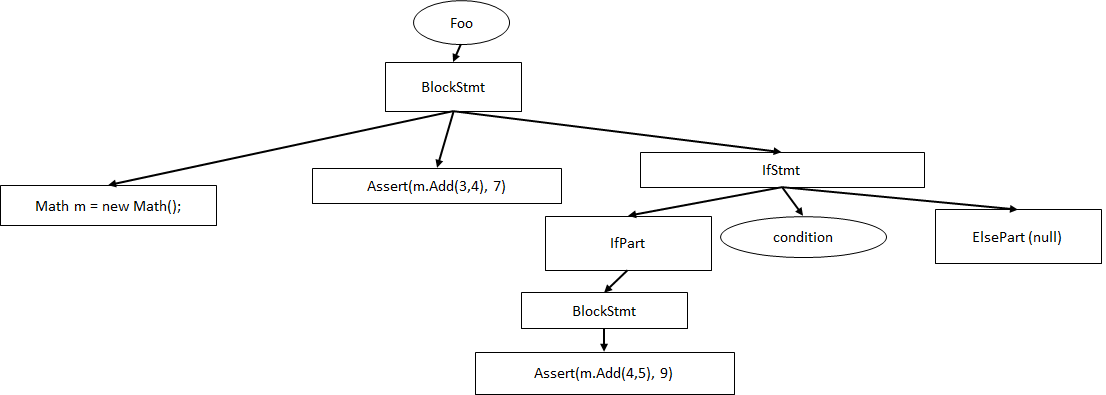
\includegraphics[width=\textwidth]{ast_tree.png}
\caption{AST of code in Figure~\ref{fig:foo}}
\label{fig:ast}
\end{figure*}

